\section{Impresion 3D aplicada a la robotica}
\label{impresion_3D}

La impresión 3D es una técnica de fabricación basado en adición de material, donde se modela el objeto a fabricar usando algún software de diseño CAD en 3D y se van añadiendo capas de material para obtener el resultado. Es una tecnología que comenzó a utilizarse a mediados de los 80 y que recientemente se ha popularizado gracias a kits de menor tamaño y coste que permiten aplicaciones domésticas. Las diferentes tecnologías empleadas en este campo pueden separarse según el modo de depositar las capas de material y según el tipo de material empleado. Atendiendo al primer criterio, se encuentran  los siguientes tipos:\\

\begin{enumerate}
\item \textbf{Impresión por extrusión}: El material, por lo general filamentos termoplásticos o de metal, se hace pasar por un extrusor que aplica calor, el cual, al combinarse con la presión debida a la diferencia de sección que existe entre el filamento y la boquilla del extrusor, provoca el paso del material de solido a fluído. El cabezal se va moviendo para dar forma a la capa y, al depositarse, el material se enfría y vuelve a ser sólido. Un ejemplo se puede ver en la figura \ref{fig:impresora_extrusion}\\

\begin{figure}[H]
        \centering
        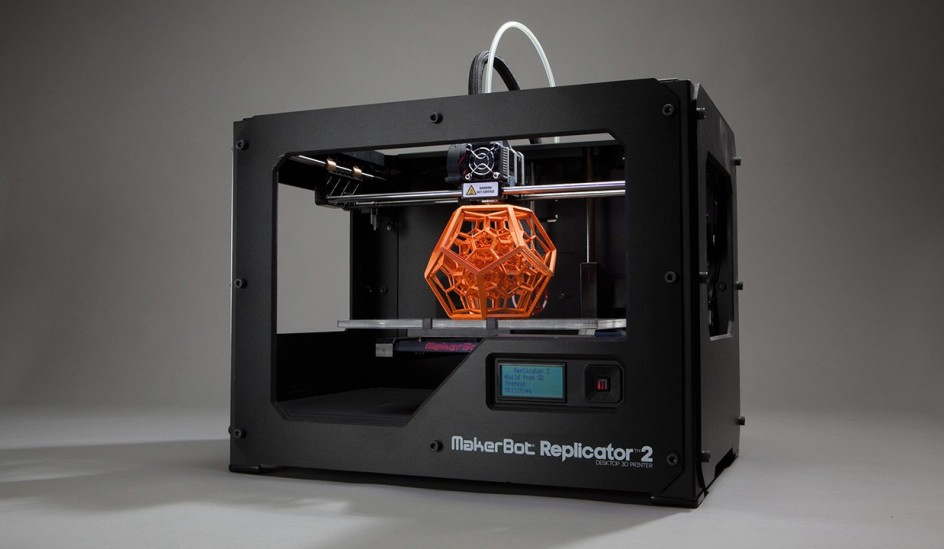
\includegraphics[width=0.4\textwidth]{images/impresion_por_extrusion.jpg}
        \caption{Impresora 3D por extrusión}
        \label{fig:impresora_extrusion}
\end{figure} 

\item \textbf{Impresión por fusión de material granulado}: Al igual que en el caso anterior, el objeto a obtener se fabrica también a base de ir añadiendo capas, solo que en este caso lo que se hace es depositar sobre la base de trabajo un material fusible y fundir aquellas partes que interesan. Una vez formada la capa, esta baja y se extiende por encima una nueva capa de material, y así sucesivamente hasta que se termine la pieza. Dependiendo del método empleado para fundir el material, se puede encontrar la sinterización selectiva por láser, que calienta el fundente hasta que las partículas se agrupan debido al proceso de sinterización, la fusión selectiva por láser, que funde completamente el material para formar la capa, y la fusión por rayos de electrones, que se usa para la fabricación de piezas metálicas, fundiendo las partículas de metal usando un rayo de electrones en el vacío. En la figura \ref{fig:impresora_extrusion} se ve una impresora de este tipo\\

\begin{figure}[H]
        \centering
        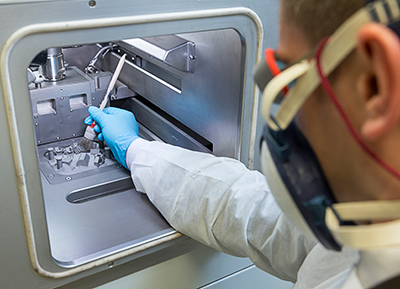
\includegraphics[width=0.4\textwidth]{images/impresion_fusion.jpg}
        \caption{Impresora 3D por fusión de material}
        \label{fig:impresora_extrusion}
\end{figure} 

\item \textbf{Impresión por laminación}: Técnica consistente en la fabricación de piezas 3D en papel, cortando la forma de la capa en cada hoja y posteriormente uniendolas todas, aplicando un adhesivo y presión.

\item \textbf{Impresión por fotopolimerización}: Se fabrica la pieza sometiendo a un polímero fotosensible a una emisión controlada de luz que provoca que se solidifique la capa. Una vez hecho esto, la base de impresión desciende, y se pasa a trabajar sobre la siguiente capa, continuando con este proceso hasta que se haya terminado el objeto. Una impresora de este tipo se puede ver en la figura \ref{fig:impresora_dlp}. Para imprimir piezas con una gran precisión (para aplicaciones de microfabricación) se puede usar la técnica de fotopolimerización por absorción de fotones. Se usa un láser para repasar la pieza sobre un bloque de resina, la cual se endurece solo en aquellas zonas donde el láser ha hecho contacto.\\

\begin{figure}[H]
        \centering
        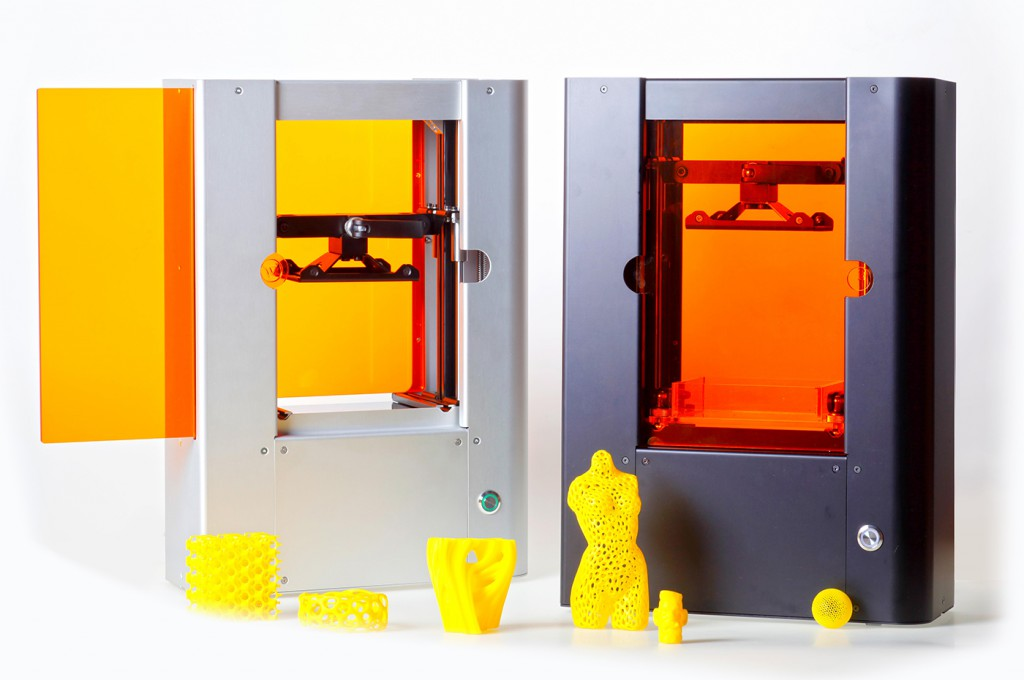
\includegraphics[width=0.4\textwidth]{images/impresion_dlp.jpg}
        \caption{Impresora 3D por fotopolimerización}
        \label{fig:impresora_dlp}
\end{figure} 
    
\end{enumerate}

Aunque esta tecnología lleva años en uso, desde hace unos años se ha producido una gran expansión con la aparición de sistemas de impresión 3D que pueden ser construídos de forma casera a un bajo coste. Esto ha dado un empujón de forma indirécta a la robótica, ya que permite diseñar y fabricar prototipos de forma rápida y cómoda, acercando este campo a todos los públicos. Usando un software de diseño asistido por ordenador, se generan unos planos en 3D de las piezas necesarias para el montaje, se imprimen y, con un controlador adecuado (hoy en día existen opciones de uso bastante general, como puede ser el caso de Aruino), servomotores y sensores comunes, se obtiene un robot simple sobre el que se puede seguir trabajando y desarrollando proyectos.  

 